\documentclass{article}
\usepackage{graphicx} % Required for inserting images

\title{Labwork 3 Advanced Programming for HPC}
\author{Ta Quang Hieu - M22ICT002}
\date{October 2023}

\begin{document}
	
	\maketitle
	
	\section{The problem}
	Labwork 5: Gaussian Blur Convolution
	
	Figure ~\ref{fig:python} the image that I used in this labwork:
	
	\begin{figure}
		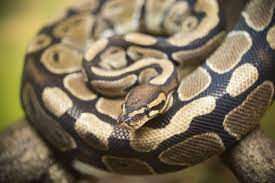
\includegraphics[width=\linewidth]{python.jpg}
		\caption{A python in rgb.}
		\label{fig:python}
	\end{figure}
	
	\section{Using GPU - not using shared memory}
	This is the kernel that I used to applying blur filter in an image not using shared memory:
	\begin{verbatim}
		# Define a Numba CUDA kernel for grayscale conversion
		@cuda.jit
		def gaussian_blur(src, dst):
		tidx, tidy = cuda.grid(2)
		
		if tidx < src.shape[0] and tidy < src.shape[1]: # because this will run through each pixel so don't need to restart
		# tidx = cuda.threadIdx.x + cuda.blockIdx.x * cuda.blockDim.x
		# tidy = cuda.threadIdx.y + cuda.blockIdx.y * cuda.blockDim.y
		total_weight = 0.0
		weighted_sum_r = 0.0
		weighted_sum_g = 0.0
		weighted_sum_b = 0.0
		for i in range(-3, 4):
		for j in range(-3, 4):
		if (tidx + i) >= 0 and (tidx + i) < src.shape[0] and (tidy + j) >= 0 and (tidy + j) < src.shape[1]:
		pixel_r = src[tidx + i, tidy + j, 0]
		pixel_g = src[tidx + i, tidy + j, 1]
		pixel_b = src[tidx + i, tidy + j, 2]
		weight = gaussian_filter[i + 3][j + 3]
		weighted_sum_r += pixel_r * weight
		weighted_sum_g += pixel_g * weight
		weighted_sum_b += pixel_b * weight
		total_weight += weight
		dst[tidx, tidy, 0] = np.uint8(weighted_sum_r / total_weight)
		dst[tidx, tidy, 1] = np.uint8(weighted_sum_g / total_weight)
		dst[tidx, tidy, 2] = np.uint8(weighted_sum_b / total_weight)
	\end{verbatim}
	
	Figure ~\ref{fig:gpu_python} is the result produced not using shared memory:
	
	\begin{figure}
		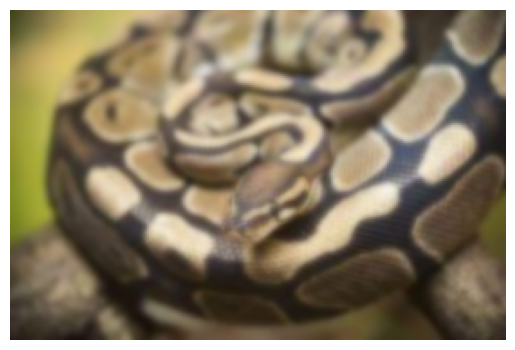
\includegraphics[width=\linewidth]{gpu_python.png}
		\caption{A blur filter - not shared.}
		\label{fig:gpu_python}
	\end{figure}
	
	\subsection{Block size vs time}
	This is the result that I take block size from 2\^1 to 2\^5:
	\begin{verbatim}
		[0.008905410766601562,
		0.0019030570983886719,
		0.0017082691192626953,
		0.0013670921325683594,
		0.0015041828155517578]
	\end{verbatim}
	Which will turn into a plot like in Figure ~\ref{fig:plot_not_shared}:
	\begin{figure}
		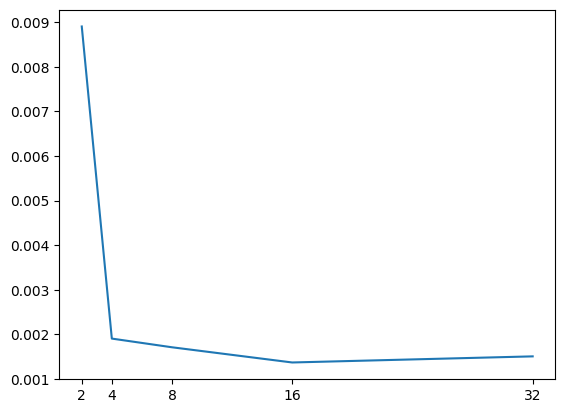
\includegraphics[width=\linewidth]{plot_not_shared.png}
		\caption{Time vs block - not shared.}
		\label{fig:plot_not_shared}
	\end{figure}
	
	\section{Using GPU - using shared memory}
	This is the script that I used to apply blur filter using shared memory:
	\begin{verbatim}
		# Define a Numba CUDA kernel for grayscale conversion
		@cuda.jit
		def gaussian_blur_shared(src, dst):
		tidx, tidy = cuda.grid(2)
		
		if tidx < src.shape[0] and tidy < src.shape[1]:
		total_weight = 0.0
		weighted_sum_r = 0.0
		weighted_sum_g = 0.0
		weighted_sum_b = 0.0
		# filter_shared = cuda.shared.array(shape=(7, 7), dtype=numba.float32)  # Define shared memory for the filter
		# tidx_s = cuda.threadIdx.x
		# tidy_s = cuda.threadIdx.y
		# filter_shared[tidx_s, tidy_s] = filter[tidx_s, tidy_s]
		# cuda.syncthreads()  # Synchronize threads to ensure filter is loaded
		# cuda.shared.array((cuda.blockDim.x, cuda.blockDim.y),numba.uint8)
		tile = cuda.shared.array((7, 7), numba.uint8)  # Define the shared memory for the filter
		# the error was due to np.type here
		# tidx_s = cuda.threadIdx.x + cuda.blockIdx.x * cuda.blockDim.x
		# tidy_s = cuda.threadIdx.y + cuda.blockIdx.y * cuda.blockDim.y
		# tile[cuda.threadIdx.x, cuda.threadIdx.y] = filter[tidx_s, tidy_s]
		tile[cuda.threadIdx.x, cuda.threadIdx.y] = gaussian_filter[cuda.threadIdx.x, cuda.threadIdx.y]
		
		cuda.syncthreads()  # Synchronize threads to ensure filter is loaded
		
		for i in range(-3, 4):
		for j in range(-3, 4):
		if (tidx + i) >= 0 and (tidx + i) < src.shape[0] and (tidy + j) >= 0 and (tidy + j) < src.shape[1]:
		pixel_r = src[tidx + i, tidy + j, 0]
		pixel_g = src[tidx + i, tidy + j, 1]
		pixel_b = src[tidx + i, tidy + j, 2]
		weight = tile[i + 3, j + 3]
		weighted_sum_r += pixel_r * weight
		weighted_sum_g += pixel_g * weight
		weighted_sum_b += pixel_b * weight
		total_weight += weight
		dst[tidx, tidy, 0] = np.uint8(weighted_sum_r / total_weight)
		dst[tidx, tidy, 1] = np.uint8(weighted_sum_g / total_weight)
		dst[tidx, tidy, 2] = np.uint8(weighted_sum_b / total_weight)
	\end{verbatim}
	
	About grid size, It must be rectangular; otherwise, the image will be cropped for some pixels.
	
	Figure ~\ref{fig:gpu_python_shared} is the result produced by GPU - using shared memory:
	
	\begin{figure}
		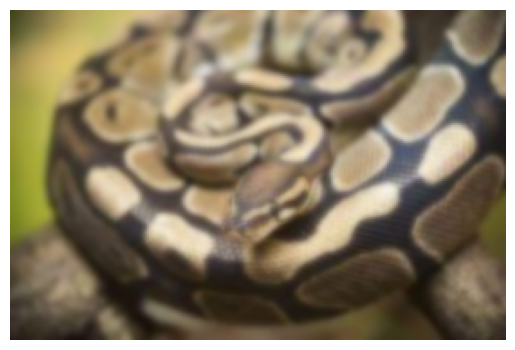
\includegraphics[width=\linewidth]{gpu_python_shared.png}
		\caption{A blur filter - shared.}
		\label{fig:gpu_python_shared}
	\end{figure}
	
	\subsection{Block size vs time}
	This is the result that I take block size from 2\^1 to 2\^5:
	\begin{verbatim}
		[0.006932973861694336,
		0.002340078353881836,
		0.0017325878143310547,
		0.0017278194427490234,
		0.0035636425018310547]
	\end{verbatim}
	Which will turn into a plot like in Figure ~\ref{fig:plot_shared}:
	\begin{figure}
		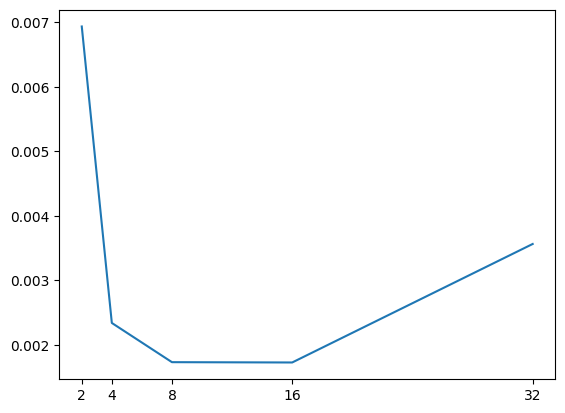
\includegraphics[width=\linewidth]{plot_shared.png}
		\caption{Time vs block - shared memory.}
		\label{fig:plot_shared}
	\end{figure}
	
	I can only run to 32*32 block size with 2d, and as we can observe using 2bd block size makes the program run faster.
	
\end{document}
